\documentclass[letterpaper]{article}
\usepackage[margin=1in]{geometry}
\usepackage[utf8]{inputenc}
\usepackage{textcomp}
\usepackage{amssymb}
\usepackage{natbib}
\usepackage{graphicx}
\usepackage{gensymb}
\usepackage{amsthm, amsmath, mathtools}
\usepackage[dvipsnames]{xcolor}
\usepackage{enumerate}
\usepackage{mdframed}
\usepackage[most]{tcolorbox}
\usepackage{csquotes}
% https://tex.stackexchange.com/questions/13506/how-to-continue-the-framed-text-box-on-multiple-pages

\tcbuselibrary{theorems}

\newcommand{\R}{\mathbb{R}}
\newcommand{\Z}{\mathbb{Z}}
\newcommand{\N}{\mathbb{N}}
\newcommand{\Q}{\mathbb{Q}}
\newcommand{\C}{\mathbb{C}}
\newcommand{\code}[1]{\texttt{#1}}
\newcommand{\mdiamond}{$\diamondsuit$}
\newcommand{\PowerSet}{\mathcal{P}}
\newcommand{\Mod}[1]{\ (\mathrm{mod}\ #1)}
\DeclareMathOperator{\lcm}{lcm}

%\newtheorem*{theorem}{Theorem}
%\newtheorem*{definition}{Definition}
%\newtheorem*{corollary}{Corollary}
%\newtheorem*{lemma}{Lemma}
\newtheorem*{proposition}{Proposition}


\newtcbtheorem[number within=section]{theorem}{Theorem}
{colback=green!5,colframe=green!35!black,fonttitle=\bfseries}{th}

\newtcbtheorem[number within=section]{definition}{Definition}
{colback=blue!5,colframe=blue!35!black,fonttitle=\bfseries}{def}

\newtcbtheorem[number within=section]{corollary}{Corollary}
{colback=yellow!5,colframe=yellow!35!black,fonttitle=\bfseries}{cor}

\newtcbtheorem[number within=section]{lemma}{Lemma}
{colback=red!5,colframe=red!35!black,fonttitle=\bfseries}{lem}

\newtcbtheorem[number within=section]{example}{Example}
{colback=white!5,colframe=white!35!black,fonttitle=\bfseries}{def}

\newtcbtheorem[number within=section]{note}{Important Note}{
        enhanced,
        sharp corners,
        attach boxed title to top left={
            xshift=-1mm,
            yshift=-5mm,
            yshifttext=-1mm
        },
        top=1.5em,
        colback=white,
        colframe=black,
        fonttitle=\bfseries,
        boxed title style={
            sharp corners,
            size=small,
            colback=red!75!black,
            colframe=red!75!black,
        } 
    }{impnote}
\usepackage[utf8]{inputenc}
\usepackage[english]{babel}
\usepackage{fancyhdr}
\usepackage[hidelinks]{hyperref}

\pagestyle{fancy}
\fancyhf{}
\rhead{CSE 105}
\chead{Wednesday, January 05, 2022}
\lhead{Lecture 2}
\rfoot{\thepage}

\setlength{\parindent}{0pt}

\begin{document}

\section{Finite Automata (1.1, Continued)}
This continues from the notes from Monday, January 3.

\subsection{Formal Definition of Computation}
To review, let $M = (Q, \Sigma, \delta, q_0, F)$ be a finite automaton and let $w = w_1 w_2 \dots w_n$ be a string where each $w_i \in \Sigma$. Then, we say that $M$ accepts $w$ if a sequence of states $r_0, r_1, \dots, r_n$ in $Q$ exists with three conditions: 
\begin{enumerate}
    \item $r_0 = q_0$: The machine starts in the start state. 
    \item $\delta(r_i, w_{i + 1}) = r_{i + 1}$, for $i = 0, \dots, n - 1$: The machine goes from state to state according to the transition function. 
    \item $r_n \in F$: The machine accepts its input if it ends up in an accept state. 
\end{enumerate}
In particular, we say that $M$ recognizes language $A$ if $A = \{w \mid M \text{ accepts } w\}$.
\begin{definition}{Regular Language}{}
    A language is called a \textbf{regular language} if some finite automaton recognizes it.
\end{definition}

\subsubsection{Example 1: State Machine}
Recall, for example, our state machine $B_3$ in the previous lecture notes. If $w$ was the string:
\begin{verbatim}
    10 RESET 22 RESET 012
\end{verbatim}
Then, $M_5$ accepts $w$ according to the formal definition of computation because the sequence of states it enters when computing on $w$ is: 
\[q_0, q_1, q_1, q_0, q_2, q_1, q_0, q_0, q_1, q_0\]
In particular:
\begin{enumerate}
    \item The machine starts in the start state as expected. 
    \item The machine goes from state to state as expected. 
    \item The machine ends at the accept state. 
\end{enumerate}

\subsection{Designing Finite Automata}
A helpful approach when designing various types of automata is: 
\begin{mdframed}[]
    \emph{Put yourself in the place of the machine you are trying to design and then see how you would go about performing the machine's task.}
\end{mdframed} 
Suppose you are given some language and want to design a finite automaton that recognizes it. Given some input string, your goal is to determine if it is a member of the language the automaton is supposed to recognize. However, you can only see each symbol one at a time; after each symbol, you need to decide whether the string seen is in the language. The hardest part is that you need to figure out what you need to remember about the string as you are reading it. Remember: you only have a finite number of states, which means finite memory (hence, \emph{finite} automata). 

\subsubsection{Example 1: Designing a Finite Automaton}
Given $\Sigma = \{\code{0, 1}\}$, suppose we need to create a finite automaton $E_2$ that recognizes the regular language of all strings that contain \code{001} as a substring. For example, \code{001}, \code{1001}, \code{0010}, \code{111111001111101} are all in the language; however, \code{0000} and \code{11} are not.

\bigskip

Well, the first thing we can do is create the set of states that will result in an \code{ACCEPT} state. This is as simple as:
\begin{center}
    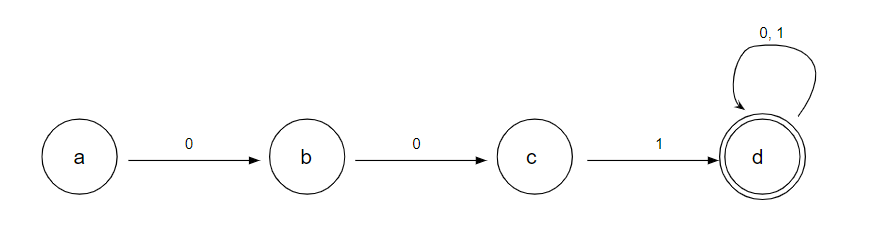
\includegraphics[scale=0.6]{../assets/state_1.png}
\end{center}
Here, it's clear that a string like \code{001} will result in an \code{ACCEPT} state. Now, we need to account for any other strings. In particular, we need to account for several different possibilities:
\begin{itemize}
    \item We haven't seen any symbols associated with the pattern (e.g. we start with \code{1}s, or we saw a \code{0} and then a \code{1}). 
    \item We just saw \code{0}.
    \item We just saw \code{00}.
    \item We have seen the pattern \code{001}.
\end{itemize}
This gives us the automaton:
\begin{center}
    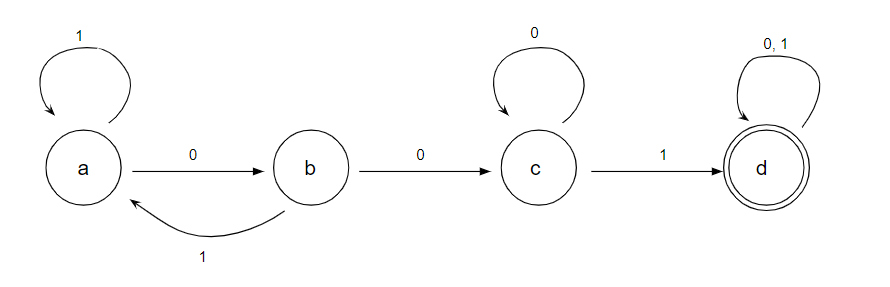
\includegraphics[scale=0.6]{../assets/state_2.png}
\end{center}

\subsection{The Regular Operations}
In arithmetic, the basic objects are numbers and the tools are operations for manipulating them (e.g. $+$ or $\times$). In the theory of computation, the objects are languages and the tools include operations designed for manipulating them. We call these \textbf{regular operations}.

\begin{definition}{}{}
    Let $A$ and $B$ be languages. We define the regular operations \textbf{union}, \textbf{concatenation}, and \textbf{star} as follows: 
    \begin{itemize}
        \item \textbf{Union:} $A \cup B = \{x \mid x \in A \text{ or } x \in B\}$.
        \item \textbf{Concatenation:} $A \circ B = \{xy \mid x \in A \text{ and } y \in B\}$
        \item \textbf{Star:} $A^* = \{x_1 x_2 \dots x_k \mid k \geq 0 \text{ and each } x_i \in A\}$
    \end{itemize}
\end{definition}
\textbf{Remarks:}
\begin{itemize}
    \item The union operation simply takes all strings in both $A$ and $B$ and puts them together into one language.
    \item The concatenation operation attaches a string from $A$ in front of a string from $B$ in \emph{all possible ways to get the strings in the new language}.
    \item The star operation attaches any number of strings in $A$ together to get a string in the new language. Note that \emph{any number} includes 0, so the empty string $\epsilon$ is always in $A^*$.
\end{itemize}

\subsubsection{Example 1: String Manipulation}
Suppose $\Sigma = \{\code{a, b, ..., z}\}$ is the standard 26 letters. Define the two languages to be:
\[A = \{\code{good, bad}\}\]
\[B = \{\code{boy, girl}\}\]
Then: 
\begin{itemize}
    \item $A \cup B = \{\code{good, bad, boy, girl}\}$
    \item $A \circ B = \{\code{goodboy, goodgirl, badboy, badgirl}\}$
    \item $A^* = \{\epsilon, \code{good, bad, goodgood, goodbad, badgood, badbad, goodgoodgood, ...}\}$
\end{itemize}

\subsection{Properties of Regular Operations}
\begin{theorem}{}{}
    The class of regular languages is closed under the union operation.
\end{theorem}
\textbf{Remark:} In other words, if $A_1$ and $A_2$ are regular language, so is $A_1 \cup A_2$.

\begin{mdframed}[]
    \begin{proof}
        The proof is left for another day.
    \end{proof}
\end{mdframed}

\begin{theorem}{}{}
    The class of regular languages is closed under the concatenation operation.
\end{theorem}
\textbf{Remark:} In other words, if $A_1$ and $A_2$ are regular language, then so is $A_1 \circ A_2$.

\begin{mdframed}[]
    \begin{proof}
        The proof is left for another day.
    \end{proof}
\end{mdframed}

\subsection{Justifying DFAs}
To prove that the DFA that we build, $M$, actually recognizes the language $L$, we ask the following questions: 
\begin{enumerate}
    \item Is every string accepted by $M$ in $L$?
    \item Is every string from $L$ accepted by $M$?\footnote{The contrapositive version is: Is every string rejected by $M$ not in $L$?}
\end{enumerate}
A string is accepted by a DFA when: 
\[ L(M) = \{ w \mid \delta^{*}(q_0, w) \in F \} \]
Where $\delta^*$ is defined by: 
\[\delta^{*}(q, w) = \begin{cases}
    q & w = \epsilon \\ 
    \delta(q, c) & w = c, c \in \Sigma \\ 
    \delta^{*}(\delta(q, c), w') & w \subset w', c \in \Sigma, w' \in \Sigma^*
\end{cases}\]


\end{document}